% Modelo de datos (PostgreSQL / Supabase) — SmartSupply (estado 2026-09)
\documentclass[tikz, border=14pt]{standalone}
\usepackage[utf8]{inputenc}
\usepackage[T1]{fontenc}
\usepackage{helvet}
\renewcommand{\familydefault}{\sfdefault}
\usetikzlibrary{positioning, arrows.meta, shapes.multipart}

\tikzset{
  tbl/.style={rectangle split, rectangle split parts=2, rectangle split part fill={black!15, white},
    draw, line width=0.8pt, text width=5.3cm, font=\footnotesize\sffamily, align=left,
    inner sep=4pt, anchor=north},
  fk/.style={line width=0.8pt, -{Latex[length=2.3mm]}},
}
\newcommand{\pk}[2]{\underline{PK}\ \textbf{#1} : #2\\}
\newcommand{\fk}[2]{FK\ #1 : #2\\}
\newcommand{\cl}[2]{\phantom{FK}\ #1 : #2\\}
\newcommand{\hd}[1]{\centering\small\textbf{#1}}

\begin{document}
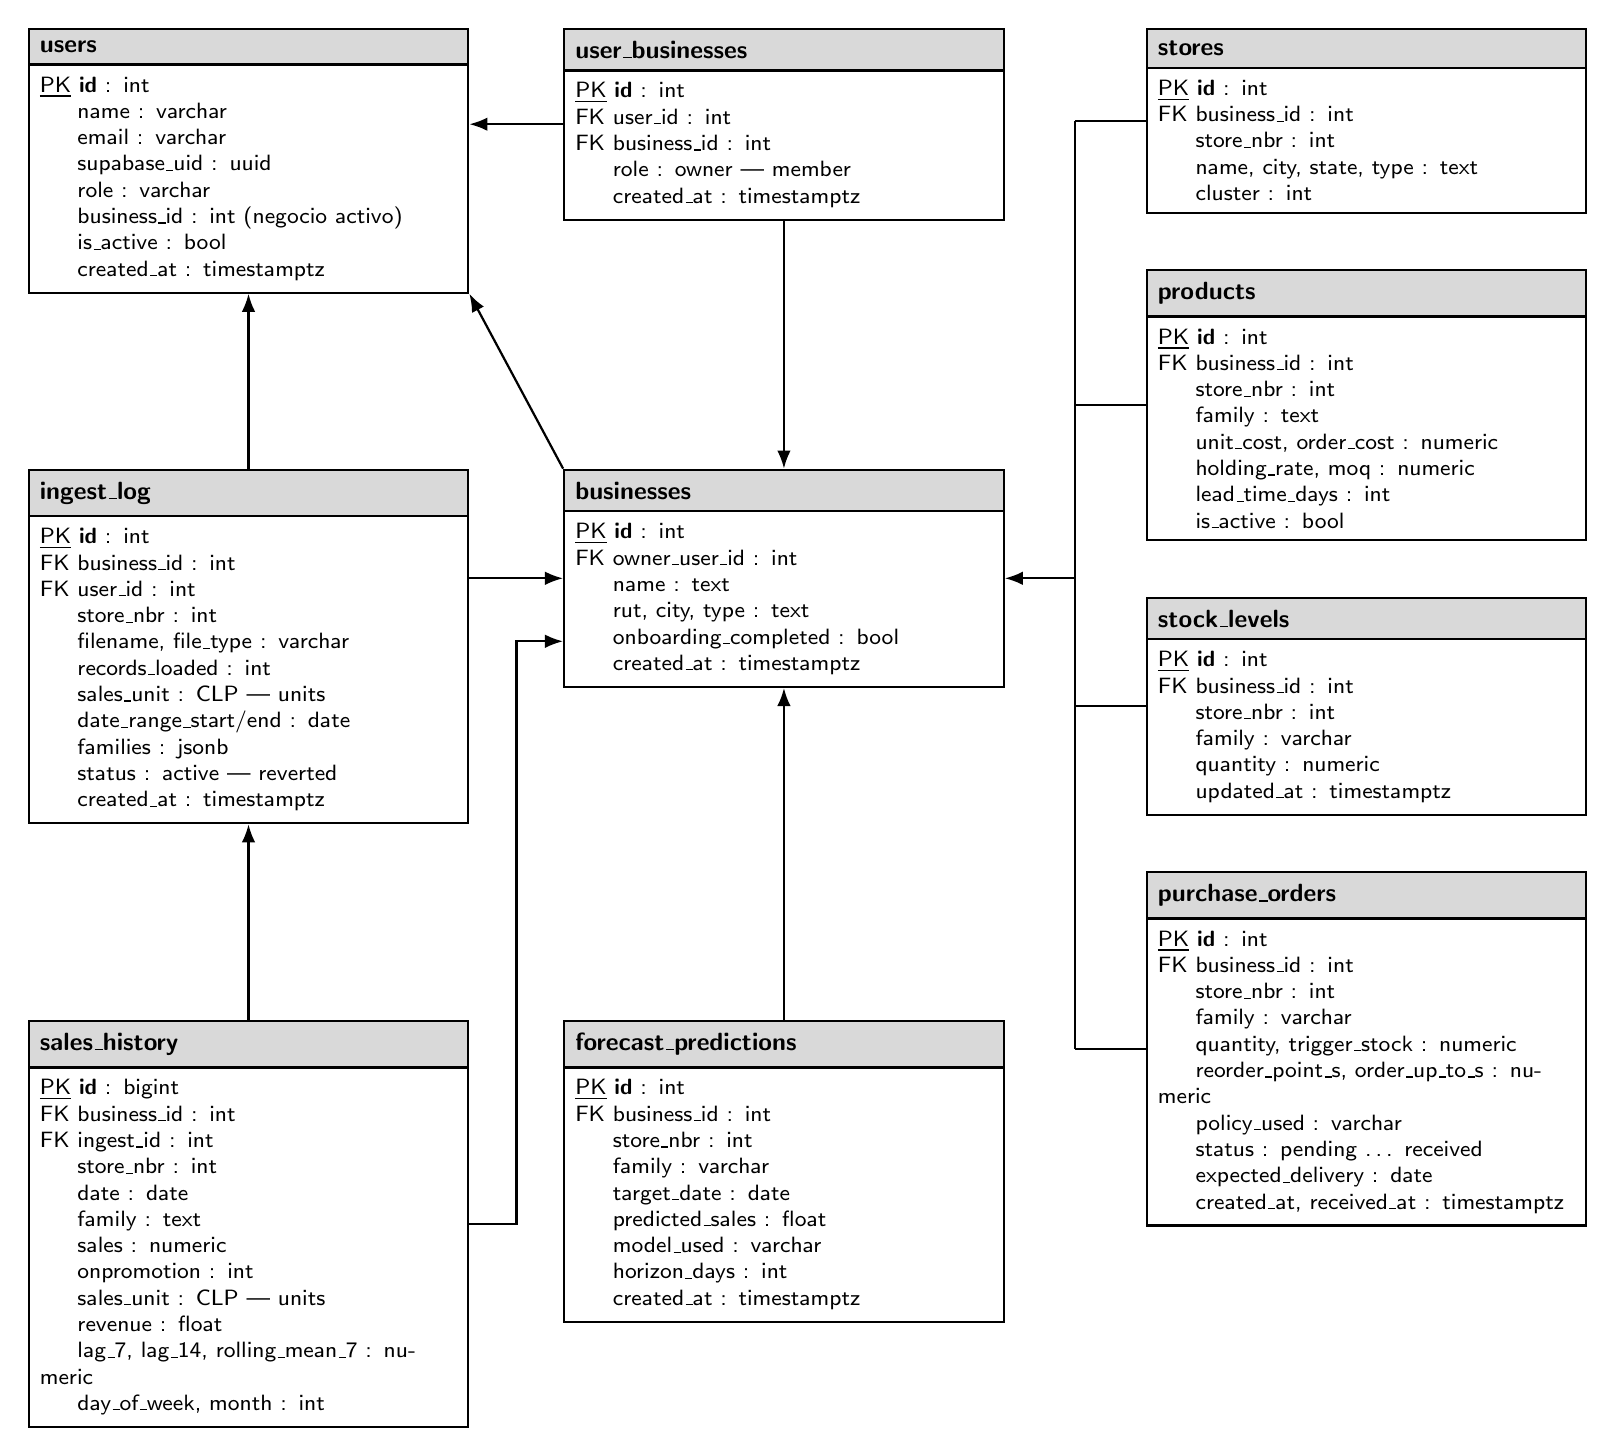
\begin{tikzpicture}[font=\sffamily]

% ── Columna 0 ───────────────────────────────────────────────
\node[tbl] (users) at (0, 0) {\hd{users}\nodepart{two}
  \pk{id}{int}
  \cl{name}{varchar}
  \cl{email}{varchar}
  \cl{supabase\_uid}{uuid}
  \cl{role}{varchar}
  \cl{business\_id}{int (negocio activo)}
  \cl{is\_active}{bool}
  \cl{created\_at}{timestamptz}};

\node[tbl] (ingest) at (0, -5.6) {\hd{ingest\_log}\nodepart{two}
  \pk{id}{int}
  \fk{business\_id}{int}
  \fk{user\_id}{int}
  \cl{store\_nbr}{int}
  \cl{filename, file\_type}{varchar}
  \cl{records\_loaded}{int}
  \cl{sales\_unit}{CLP | units}
  \cl{date\_range\_start/end}{date}
  \cl{families}{jsonb}
  \cl{status}{active | reverted}
  \cl{created\_at}{timestamptz}};

\node[tbl] (sales) at (0, -12.6) {\hd{sales\_history}\nodepart{two}
  \pk{id}{bigint}
  \fk{business\_id}{int}
  \fk{ingest\_id}{int}
  \cl{store\_nbr}{int}
  \cl{date}{date}
  \cl{family}{text}
  \cl{sales}{numeric}
  \cl{onpromotion}{int}
  \cl{sales\_unit}{CLP | units}
  \cl{revenue}{float}
  \cl{lag\_7, lag\_14, rolling\_mean\_7}{numeric}
  \cl{day\_of\_week, month}{int}};

% ── Columna 1 ───────────────────────────────────────────────
\node[tbl] (ub) at (6.8, 0) {\hd{user\_businesses}\nodepart{two}
  \pk{id}{int}
  \fk{user\_id}{int}
  \fk{business\_id}{int}
  \cl{role}{owner | member}
  \cl{created\_at}{timestamptz}};

\node[tbl] (biz) at (6.8, -5.6) {\hd{businesses}\nodepart{two}
  \pk{id}{int}
  \fk{owner\_user\_id}{int}
  \cl{name}{text}
  \cl{rut, city, type}{text}
  \cl{onboarding\_completed}{bool}
  \cl{created\_at}{timestamptz}};

\node[tbl] (fp) at (6.8, -12.6) {\hd{forecast\_predictions}\nodepart{two}
  \pk{id}{int}
  \fk{business\_id}{int}
  \cl{store\_nbr}{int}
  \cl{family}{varchar}
  \cl{target\_date}{date}
  \cl{predicted\_sales}{float}
  \cl{model\_used}{varchar}
  \cl{horizon\_days}{int}
  \cl{created\_at}{timestamptz}};

% ── Columna 2 (dependen de businesses) ──────────────────────
\node[tbl] (stores) at (14.2, 0) {\hd{stores}\nodepart{two}
  \pk{id}{int}
  \fk{business\_id}{int}
  \cl{store\_nbr}{int}
  \cl{name, city, state, type}{text}
  \cl{cluster}{int}};

\node[tbl, below=0.7cm of stores] (prod) {\hd{products}\nodepart{two}
  \pk{id}{int}
  \fk{business\_id}{int}
  \cl{store\_nbr}{int}
  \cl{family}{text}
  \cl{unit\_cost, order\_cost}{numeric}
  \cl{holding\_rate, moq}{numeric}
  \cl{lead\_time\_days}{int}
  \cl{is\_active}{bool}};

\node[tbl, below=0.7cm of prod] (stock) {\hd{stock\_levels}\nodepart{two}
  \pk{id}{int}
  \fk{business\_id}{int}
  \cl{store\_nbr}{int}
  \cl{family}{varchar}
  \cl{quantity}{numeric}
  \cl{updated\_at}{timestamptz}};

\node[tbl, below=0.7cm of stock] (po) {\hd{purchase\_orders}\nodepart{two}
  \pk{id}{int}
  \fk{business\_id}{int}
  \cl{store\_nbr}{int}
  \cl{family}{varchar}
  \cl{quantity, trigger\_stock}{numeric}
  \cl{reorder\_point\_s, order\_up\_to\_s}{numeric}
  \cl{policy\_used}{varchar}
  \cl{status}{pending \dots\ received}
  \cl{expected\_delivery}{date}
  \cl{created\_at, received\_at}{timestamptz}};

% ── Relaciones (FK -> PK) ───────────────────────────────────
\draw[fk] (ub.west) -- (users.east |- ub.west);
\draw[fk] (ub.south) -- (biz.north);
\draw[fk] (biz.north west) -- (users.south east);
\draw[fk] (ingest.north) -- (users.south);
\draw[fk] (ingest.east |- biz.west) -- (biz.west);
\draw[fk] (sales.north) -- (ingest.south);
\draw[fk] (sales.east) -- ++(0.6,0) |- ([yshift=-8mm]biz.west);
\draw[fk] (fp.north) -- (biz.south);

% Bus comun hacia businesses para la columna 2
\coordinate (bus) at (10.5, 0);
\foreach \t in {stores, prod, stock, po} {
  \draw[line width=0.8pt] (\t.west) -- (bus |- \t.west);
}
\draw[line width=0.8pt] (bus |- stores.west) -- (bus |- po.west);
\draw[fk] (bus |- biz.east) -- (biz.east);

\end{tikzpicture}
\end{document}
